\documentclass[a4paper]{article}

\usepackage[pages=all, color=black, position={current page.south}, placement=bottom, scale=1, opacity=1, vshift=5mm]{background}
\usepackage[margin=1in]{geometry}

% AMS Packages
\usepackage{amsmath}
\usepackage{amsthm}
\usepackage{amssymb}

% Unicode
\usepackage[utf8]{inputenc}
\usepackage{hyperref}
\hypersetup{
	unicode,
	pdfauthor={Swarnava Mandal, Saumitra Prasad Kulkarni, Ayush Singh},
	pdftitle={Music Genre Classification},
	pdfsubject={Classification using ML},
	pdfkeywords={music genre, classification, machine learning, Random Forest, neural network},
	pdfproducer={LaTeX},
	pdfcreator={pdflatex}
}

% Natbib
\usepackage[sort&compress,numbers,square]{natbib}
\bibliographystyle{mplainnat}

% Theorem
\theoremstyle{plain}
\newtheorem{theorem}{Theorem}
\theoremstyle{definition}
\newtheorem{definition}[theorem]{Definition}
\newtheorem{example}[theorem]{Example}

\usepackage{graphicx, color}
\graphicspath{{fig/}}

\usepackage{algorithm, algpseudocode}
\usepackage{mathrsfs}

\title{Music Genre Classification}
\author{Swarnava Mandal$^1$ \and Saumitra Prasad Kulkarni$^1$ \and Ayush Singh$^1$}
\date{
	$^1$IIT Jodhpur \\ \texttt{\{B23EE1072, B23EE1065, B23EE1008\}@iitj.ac.in} \\[2ex]
	\url{https://github.com/Saumi18/Music-Genre-Classification}
}

\begin{document}
\maketitle

\begin{abstract}
This project focuses on classifying music genres using a hybrid machine learning approach. We explore various models like Random Forest, SVM, ANN, and K-Nearest Neighbors (KNN), choosing the best model at end. We also include dimensionality reduction using PCA. Our implementation is from scratch and evaluated on the GTZAN dataset using metrics like accuracy and confusion matrix.
\vspace{1cm}

\noindent\textbf{Keywords:} Music Genre Classification, Random Forest, Neural Network, PCA + GMM, KNN, SVM.
\end{abstract}

\tableofcontents

\section{Introduction}
\label{sec:intro}
Music genre classification plays a vital role in music recommendation systems and audio content organization. The goal of this project is to classify music samples into predefined genres using machine learning techniques. We developed and evaluated multiple models from scratch, including KNN, Random Forest, SVM (One-vs-All), and a Neural Network. Finally, we implemented the best model with highest accuracy.

\section{Approaches Tried}
\label{sec:app}

We implemented and tested the following approaches:

\begin{enumerate}
    \item \textbf{KNN from scratch}: We implemented KNN using Euclidean distance to classify a sample based on the majority label of its closest neighbors.It is a non-parametric, instance-based learning algorithm that makes no assumptions about data distribution.The model was evaluated using different values of k to optimize classification accuracy.KNN achieved good performance on the GTZAN dataset due to its simplicity and effectiveness on clean, labeled data.
    \item \textbf{Random Forest from scratch}: We implemented a Random Forest from scratch using parallel processing and manual tree building.Each decision tree was grown using bootstrap samples and random feature selection for node splits. Gini impurity was used to determine the best splits, and trees stopped growing based on depth or purity. The model predicted outputs via majority voting across all trees, with support for both labels and probabilities. It performed robustly on the GTZAN dataset and provided interpretability while demonstrating ensemble learning's power.
    \item \textbf{Random Forest using SKLearn}: Implemented using the sklearn library with hyperparameter tuning using GridSearchCV and evaluated using Stratified K-Fold cross-validation for optimal performance. The final model was selected based on the best combination of parameters.
    \item \textbf{SVM (One-vs-All)}: We implemented a binary Support Vector Machine (SVM) from scratch using gradient descent and hinge loss.Then extended it to handle multiclass classification using the One-vs-All strategy, training one classifier per class.Each classifier distinguishes one genre from all others and makes predictions based on maximum margin separation.The model showed good interpretability and control over training dynamics via learning rate and regularization. We evaluated it using a confusion matrix, giving insights into how well each genre was distinguished.
    \item \textbf{Neural Network}: We designed a deep neural network with dropout, batch normalization, and multiple hidden layers for robust learning. It was trained using the Adam optimizer with learning rate scheduling and evaluated on a multiclass music genre dataset. The network learns complex feature interactions, improving generalization and accuracy compared to simpler models. The model achieved strong results and was visualized using a confusion matrix for class-level performance analysis. Finally, we saved the trained model for reuse, making it practical for deployment or further tuning.
    \item \textbf{(PCA + GMM)}: Applied Gaussian Mixture Model (GMM) with Expectation Maximization (EM) for clustering, using PCA for dimensionality reduction and SelectKBest for feature selection to predict music genre classification.
\end{enumerate}

Each model was evaluated on its accuracy and confusion matrix.

\section{Experiments and Results}
\label{sec:results}

\subsection{Dataset}
We used the \textbf{GTZAN dataset}, which contains 1000 audio tracks equally distributed among 10 music genres. We extracted features from 3-second audio segments using pre-processed \texttt{features\_3\_sec.csv} file.

\subsection{Experimental Setup}
\begin{itemize}
    \item Environment: Python 3.10
    \item Libraries: NumPy, Pandas, Scikit-learn (for metrics only)
    \item Custom Implementations: KNN, Random Forest, SVM, Neural Network, GMM
    \item Evaluation Metric: Accuracy, Confusion Matrix
\end{itemize}

\subsection{Results Summary}

\begin{itemize}
    \item KNN Accuracy: \texttt{91\%}
\end{itemize}
\begin{figure}[H]
    \centering
    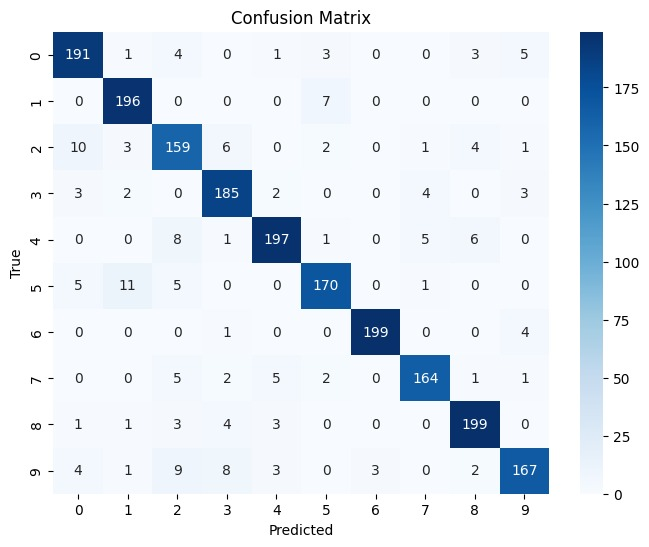
\includegraphics[width=0.6\textwidth]{knn_cm.png}
    \caption{Confusion Matrix for KNN}
\end{figure}

\begin{itemize}
    \item Random Forest Accuracy (From Scratch): \texttt{86\%}
\end{itemize}
\begin{figure}[H]
    \centering
    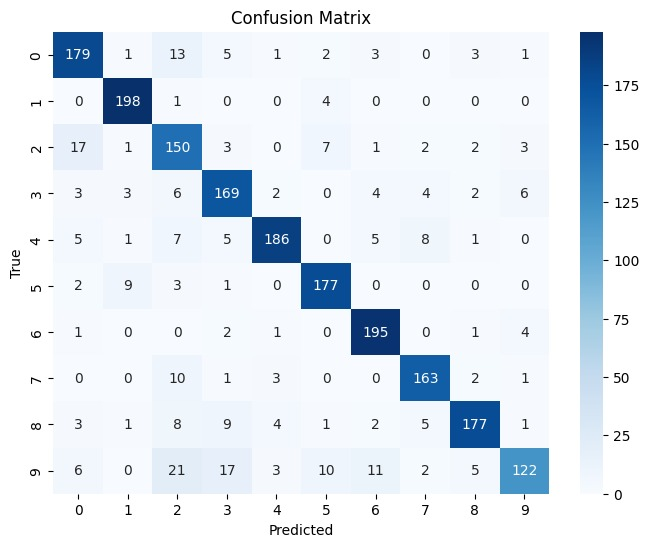
\includegraphics[width=0.6\textwidth]{rf_scratch_cm.png}
    \caption{Confusion Matrix for Random Forest (From Scratch)}
\end{figure}

\begin{itemize}
    \item Random Forest Accuracy (Using SKLearn): \texttt{89\%}
\end{itemize}

\begin{itemize}
    \item GMM Accuracy: \texttt{40\%}
\end{itemize}
\begin{figure}[H]
    \centering
    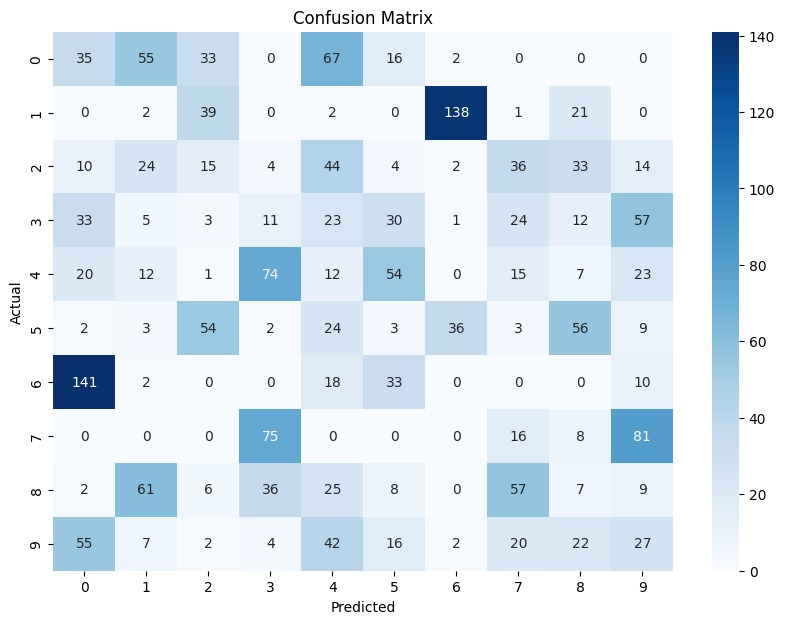
\includegraphics[width=0.6\textwidth]{gmm_cm.png}
    \caption{Confusion Matrix for GMM}
\end{figure}

\begin{itemize}
    \item SVM Accuracy: \texttt{50\%}
\end{itemize}
\begin{figure}[H]
    \centering
    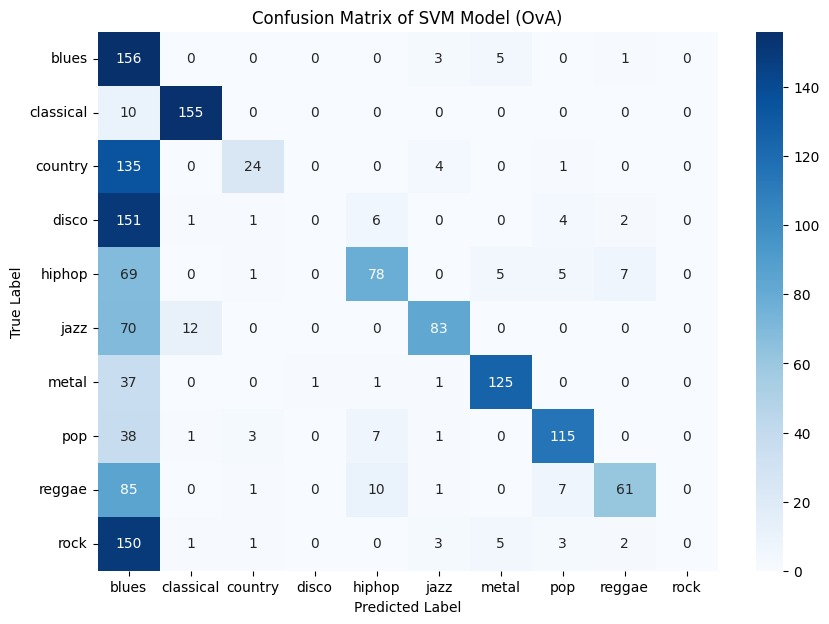
\includegraphics[width=0.6\textwidth]{svm_cm.png}
    \caption{Confusion Matrix for SVM}
\end{figure}
\begin{itemize}
    \item Neural Network Accuracy: \texttt{93.5\%}
\end{itemize}
\begin{figure}[H]
    \centering
    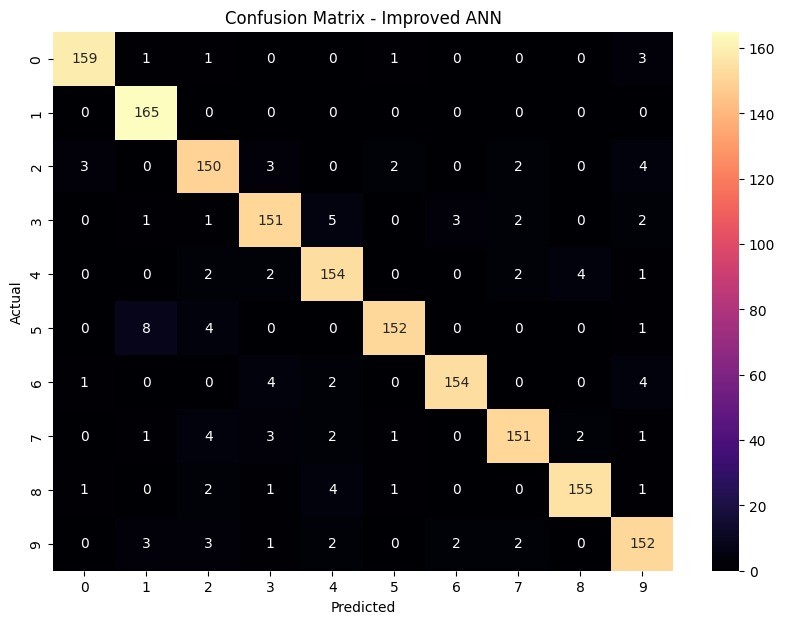
\includegraphics[width=0.6\textwidth]{nn_cm.png}
    \caption{Confusion Matrix for Neural Network}
\end{figure}

\subsection{Cloud Exploration}
During the course of this project, we also explored cloud-based platforms such as \texttt{Google Colab} and \texttt{Kaggle Kernels} for faster training and experimentation. These platforms provided access to GPU resources and enabled more efficient development and testing of deep learning models, especially the Artificial Neural Network implemented using PyTorch.


\section{Summary}
\label{sec:summary}
In this project, we explored and implemented several machine learning models for the task of music genre classification using the GTZAN dataset. Our approach began with traditional algorithms such as K-Nearest Neighbors (KNN) and Random Forest, where we not only used scikit-learn implementations but also developed a custom Random Forest model from scratch to understand the underlying mechanics. We then moved on to implement a Support Vector Machine (SVM) from scratch using a One-vs-All strategy and gradient descent optimization. To further improve classification performance, we designed and trained a feedforward Artificial Neural Network (ANN) using PyTorch, incorporating enhancements like batch normalization, dropout, and learning rate scheduling for better generalization and stability during training.Each model was evaluated using accuracy scores and confusion matrices to analyze performance. The neural network model ultimately yielded the highest accuracy of 93.5 percent, outperforming all other models. Based on these results, we selected the ANN as the final model for music genre classification.
This project demonstrates a systematic approach to model experimentation and comparison, where we not only evaluated multiple models but also fine-tuned and improved them step by step, both from theoretical and practical standpoints.

\section{Future Work}
\begin{itemize}
    \item Fine-tune model hyperparameters for better accuracy.
    \item Experiment with deep learning models (CNN, RNN).
    \item Improve feature extraction using raw audio and spectrograms.
\end{itemize}

\bibliography{refs}

\appendix

\section{Contribution of each member}
\label{sec:contribution}
\begin{enumerate}
    \item Swarnava Mandal, Ritik Singh: Implemented Custom Random Forest, and Custom KNN and performed evaluations and plotted confusion matrices, created Project Page, created Report.
    \item Kukatlapalli William Samuel, Saumitra Prasad Kulkarni: Implemented Neural Networks, PCA + GMM, created Minutes of Meeting, report, Spotlight Video.
    \item Prince Kumar, Ayush Singh: Implemented SVM, handled dataset processing, Web Demo, Spotlight Video.
\end{enumerate}

\end{document}
